% mainfile: ../../../../master.tex
\subsection{Migration of nucleic acids in agarose gel}
% The part of the label after the colon must match the file name. Otherwise,
% conditional compilation based on task labels does NOT work.
\label{task:20180201_cj3}
\tags{lab}
\authors{cj}
%\files{}
\persons{Mia Cerfonteyn} % Here, you can write the persons who attented the meeting

Because I was busy with an extraction of DNA and RNA, Mia casted the gel and ran the electrophoresis for me. 

According to figure \ref{fig:20180201_OneTaq_EMP_ARCH}, only the DNA extracted with protocol C has been amplified. It is not the results Mia and I were expecting because the Qubit measurements suggests we obtained more DNA using the Epicentre Kit. 

\begin{figure}[H] 
    \centering
    \caption{Picture of 1\% agarose gel after 50 minute-long electrophoresis migration of \gls{pcr} products obtained with \gls{emp} and \texttt{ARCH} primers and \gls{dna} extrated from surface seawater samples.}
    \label{fig:20180201_OneTaq_EMP_ARCH}
    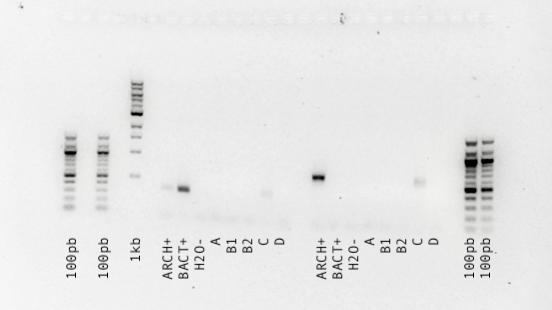
\includegraphics[width=\textwidth]{graphics/pic/20180201_OneTaq_EMP_ARCH.png}
\end{figure}

Maybe the DNA isolated with the Epicentre kit is not as pure as what we thought, which means by adding 5 \uL of DNA template in the PCR mix might also add too much contaminents, so we could try to repeat the PCR using lower quantities of template DNA which would also reduce the concentration of contaminents. 

\comment{I am not gonna repeat the PCR tonight because I have training and I know I will not be able to make it on time if I decide to start the PCR now so Mia decided to do it.}

